\documentclass[11pt]{article}
%Gummi|063|=)
\title{\textbf{Algorithms I -- supervision 6}}
\author{James Wood}
\usepackage{listings}
\usepackage{bold-extra}
\usepackage{xcolor}
\usepackage{amsmath}
\usepackage{enumitem}
\usepackage{tikz}
\usetikzlibrary{arrows}

\lstset{
  basicstyle=\small,
  basewidth=0.5em,
  frame=single,
  breaklines=true,
  %postbreak=\raisebox{0ex}[0ex][0ex]{
  %  \ensuremath{\color{red}\hookrightarrow\space}
  %}
  language=c++,
  literate=
    {<=}{{\(\leq\)}}1
    {>=}{{\(\geq\)}}1
    {&&}{{\(\wedge\)}}1
    {||}{{\(\vee\)}}1
    {->}{{\(\rightarrow\)}}1
}

\tikzset{
  treenode/.style = {align=center, inner sep=0pt, text centered,
    font=\sffamily},
  bnode/.style = {treenode, circle, white, draw=black,
    fill=black, text width=1.5em},
  rnode/.style = {treenode, circle, red, draw=red,
    text width=1.5em, very thick},
  leaf/.style = {treenode, rectangle, draw=black,
    minimum width=0.5em, minimum height=0.5em}
}

\begin{document}
\renewcommand{\labelenumi}{(\alph{enumi})}
\renewcommand{\labelenumii}{(\roman{enumii})}

\maketitle

\section{Dijkstra}
\begin{enumerate}
\item The algorithm starts at a given vertex, whose distance is marked as 0. All edges connected to this vertex are added to a priority queue, sorted by weight in ascending order (lightest first). The first vertex in the queue is then traversed, and the new vertex is given a distance equal to the weight of the edge. Its edges are then added to the queue, and the process is repeated (assigning distances equal to the weight of the edge plus the distance given to the vertex at the other end of the edge). Edges between vertices with distances already calculated are removed from the queue. Assuming a connected graph, the algorithm terminates when all vertices have been assigned a distance, or equivalently when the queue is exhausted.
\item
  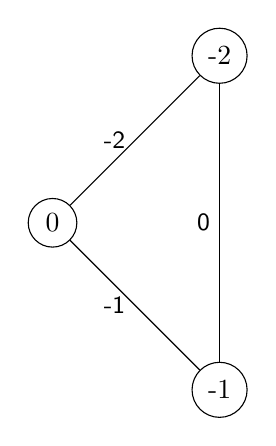
\begin{tikzpicture}[baseline={(1.base)},node distance=3cm,main node/.style={circle,draw}]
    \node[main node] (1) {-2};
    \node[main node] (2) [below left of=1] {0};
    \node[main node] (3) [below right of=2] {-1};

    \path[every node/.style={font=\sffamily\small}]
    (1) edge node [left] {-2} (2)
    (2) edge node [left] {-1} (3)
    (3) edge node [left] {0} (1);
  \end{tikzpicture}
\item Consider this graph:

  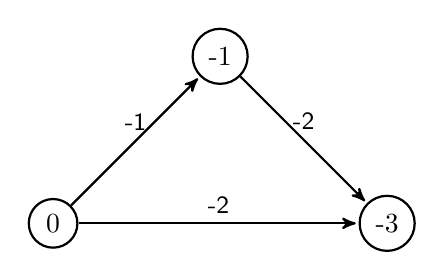
\begin{tikzpicture}[->,>=stealth',shorten >=1pt,auto,node distance=3cm,thick,main node/.style={circle,draw}]
    \node[main node] (0) {0};
    \node[main node] (1) [above right of=0] {-1};
    \node[main node] (2) [below right of=1] {-3};

    \path[every node/.style={font=\sffamily\small}]
    (0) edge node [above] {-1} (1)
    (1) edge node [above] {-2} (2)
    (0) edge node [above] {-2} (2);
  \end{tikzpicture}

  The shortest path from left to right goes via the middle node. Adding 2 to the weight of each arc gives this:

  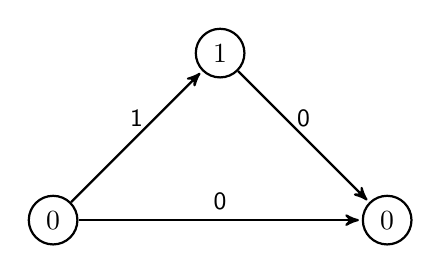
\begin{tikzpicture}[->,>=stealth',shorten >=1pt,auto,node distance=3cm,thick,main node/.style={circle,draw}]
    \node[main node] (0) {0};
    \node[main node] (1) [above right of=0] {1};
    \node[main node] (2) [below right of=1] {0};

    \path[every node/.style={font=\sffamily\small}]
    (0) edge node [above] {1} (1)
    (1) edge node [above] {0} (2)
    (0) edge node [above] {0} (2);
  \end{tikzpicture}

  The shortest path from left to right is now to go there directly. Hence, this tactic does not work.
\item
\end{enumerate}

\section{Amortized and aggregate analysis}
\begin{enumerate}
\item Amortized analysis involves finding a worst-case sequence of instructions, analyzing the complexity of the sequence and dividing the cost of the sequence by the length of the sequence, yielding an average cost for each instruction. Aggregate analysis is done by creating a measure function for the given data structure, and giving the cost of each operation as its time complexity plus the change it causes in the measure of the data structure.
\item
  \begin{enumerate}
  \item The \texttt{multipush} operation can be run on any stack, and will always have cost \(n\), where \(n\) is the length of the list of items being pushed. Hence, its amortized cost is \(O\,n\).
  \item
    \begin{minipage}[t]{\linewidth}
      \begin{lstlisting}
class Queue
    Stack front
    Stack back

    void enqueue(Item x)
        back.push(x)

    Item dequeue()
        if front.isEmpty() then
            until back.isEmpty()
                front.push(back.pop())
        return front.pop()

    Boolean isEmpty()
        return front.isEmpty() && back.isEmpty()
      \end{lstlisting}
    \end{minipage}
  \item Let \(\phi\) be a function measuring the length of \texttt{back}. \texttt{enqueue} has time cost 1 plus potential cost 1. \texttt{dequeue} has either time cost 1 plus potential cost 0, or time cost \(n+1\) plus potential cost \(-n\). \texttt{isEmpty} has time cost 1 plus potential cost 0. Each of these possibilites give linear aggregate cost, so the amortized running time of each operation is linear.
  \end{enumerate}
\end{enumerate}

\section{Linear cost}
When only a single item of an array is put out of order, bubble sort requires only two passes (one to put the element in the correct place, and another to check that the array is sorted).

\section{Disjoint-sets, linked lists and trees}
\begin{enumerate}
\item The disjoint-set data structure represents a collection of sets, with no two of those sets sharing any elements. Items can be queried as to which set they are in, and sets can be merged together (preserving all elements, since they are disjoint to each other).
\item Each subset is stored as a linked list, and these are all stored inside a linked list. This takes \(O\,n\) time to create, \(O\,n\) time to find elements and \(O\,(s+l)\) time to merge two subsets (where \(s\) is the number of subsets and \(l\) is the size of the first subset of the two being merged).
\item In Kruskal's algorithm, data representing each edge of the graph are put into a priority queue with lighter edges first. Also, data representing vertices are put into a disjoint-set data structure. Edges are taken from the priority queue and added to the output tree iff they connect vertices from different subsets. When an edge is added, the sets containing its vertices are merged. The algorithm terminates when there is only one disjoint set left.
\item At most \(|E|\) edges are chosen. If the edges are given in a sorted list (which took \(O\,(|E|\cdot\log{|E|})\) time to create), the edge is taken from the priority queue in constant time. The resulting computation consists of two \texttt{find}s and a \texttt{merge}, which combined can take \(O\,|V|\) time. In a connected graph, \(|V|\leq 2\cdot|E|\), so this is equivalent to \(O\,|E|\). Therefore, the total running time is \(O\,(|E|\cdot\log{|E|})\).
\end{enumerate}

\section{Recurrence relations}
\begin{enumerate}
\item
  \begin{aligned}
    2\cdot
  \end{aligned}
\end{enumerate}

\section{k-Anonymity}
\begin{enumerate}
\item Yes. There are an odd number of elements, so there had to be some group of three, which has a cost of at least 3. Pairings have a cost of at least 1. This solution incurred only those costs, so is optimal.
\item Let the length of the list be \(d\cdot k+r\). Partition it into \(d-1\) \(k\)-length subsequences and one \(k+r\)-length subsequence (with all subsequences made up of contiguous items), and vary the positioning of the \(k+r\)-length subsequence. Increase the values of the items in each partition to the maximum in that partition. The resulting \(d\) outputs will satisfy conditions i and ii. The final output is the output amongst these with the lowest cost (satisfying iii).

This has cost \(O\,(d\cdot n)\), because \(d\) possible outputs are processed, each taking unit time for each of the \(n\) items in them. This bound is equivalent to \(O\,(n^2)\).
\item Only consider a single intermediate result from the above algorithm.
\end{enumerate}

\end{document}